      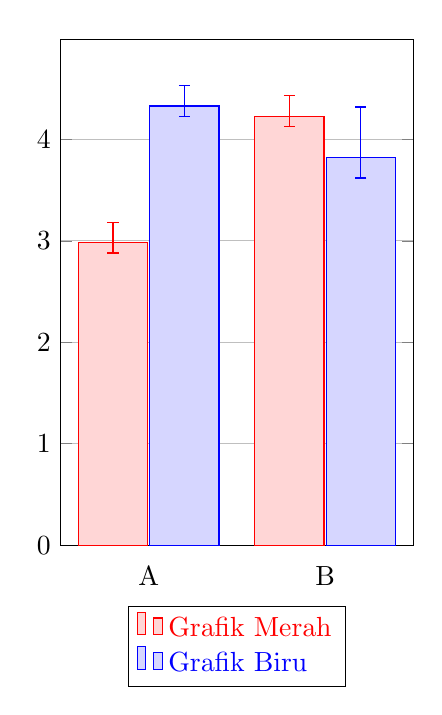
\begin{tikzpicture}
      \begin{axis}[
      width  = 0.50*\textwidth,
      height = 8cm,
      major x tick style = transparent,
      ybar=2*\pgflinewidth,
      bar width=25pt,
      ymajorgrids = true,
      symbolic x coords={A,B},
      xtick = data,
      scaled y ticks = false,
      enlarge x limits=0.50,
      ymin=0,
      legend cell align=left,
      legend style={at={(0.5,-0.12)},anchor=north},
  ]
      \addplot[red,style={fill=red!80!white!20},error bars/.cd, y dir=both, y explicit]
          coordinates {
          (A, 2.98) += (0,0.2) -= (0,0.1)
          (B,4.23) += (0,0.2) -= (0,0.1)};

      \addplot[style={blue,fill=blue!80!white!20},error bars/.cd, y dir=both, y explicit,error bar style=blue]
           coordinates {
           (A,4.33) += (0,0.2) -= (0,0.1)
           (B,3.82) += (0,0.5) -= (0,0.2)};

      \legend{\textcolor{red}{Grafik Merah}, \textcolor{blue}{Grafik Biru}}
  \end{axis}
  \end{tikzpicture}
